\documentclass[12pt]{article}
\usepackage{amsmath}
\usepackage{graphicx,psfrag,epsf}
\usepackage{enumerate}
\RequirePackage[colorlinks,citecolor=blue,urlcolor=blue]{hyperref}

\usepackage{natbib}
\usepackage{url} % not crucial - just used below for the URL 
\usepackage{commath}
%%%%%%%%%%%%%%%%%%%%%
%%%Packages from proposal
%%%%%%%%%%%%%%%%%%%%%%
\usepackage{tabularx}
\usepackage{graphics}
\usepackage{graphicx}
\usepackage{epsfig}
\usepackage{times}
\usepackage{algorithm}
\usepackage{algpseudocode}
\usepackage{pifont}
\usepackage{subcaption}
%\usepackage{graphicx}
\usepackage{float}
\usepackage[shortlabels]{enumitem}
\setlist[enumerate, 1]{1\textsuperscript{o}}
\usepackage{mathtools}
\usepackage{caption}
\usepackage{multirow}
\usepackage{bmpsize}
%\usepackage[round]{natbib}
\usepackage{caption}
\usepackage{enumitem}
\usepackage{color}
\usepackage{xcolor,colortbl}
\usepackage{amsfonts}
\usepackage{amssymb}
\usepackage{booktabs,tabulary}
\usepackage{array}
\usepackage{bm}
\usepackage{multirow}
\usepackage{fullpage}
\usepackage{enumitem}
\usepackage{lscape}
\usepackage{arash_macros}
\usepackage[titletoc,title]{appendix} 
\usepackage{bbm}
\usepackage{multirow}
\usepackage[normalem]{ulem}
\useunder{\uline}{\ul}{}
%\usepackage{slashbox}
%\usepackage{pdflscape}
%\usepackage{lscape}

\usepackage{setspace}

%%%%%%%%%%%%%%%%%%%%%%%%%%%%%%%

%\pdfminorversion=4
% NOTE: To produce blinded version, replace "0" with "1" below.
\newcommand{\blind}{0}


\usepackage[margin=1in]{geometry}
%% DON'T change margins - should be 1 inch all around.
%\addtolength{\oddsidemargin}{-.5in}%
%\addtolength{\evensidemargin}{-.5in}%
%\addtolength{\textwidth}{1in}%
%\addtolength{\textheight}{1.3in}%
%\addtolength{\topmargin}{-.8in}%
%%\DeclareMathOperator*{\argmin}{arg\,min}

\newcommand{\thh}{\widehat\theta}
\newcommand{\rhoh}{\widehat\rho}
\newcommand{\Sigt}{\widetilde{\Sigma}}
\newcommand{\rhot}{\widetilde{\rho}}
\newcommand{\tauc}{\check{\tau}}
\newcommand{\wc}{\check w}
\newcommand{\Eb}{\overline{E}}
\newcommand{\Sigh}{\widehat{\Sigma}}

\newcommand{\Expect}{{\rm I\kern-.3em E}}
\def\spacingset#1{\renewcommand{\baselinestretch}%
	{#1}\small\normalsize} \spacingset{1}

\newcommand{\aaa}[1]{\textcolor{blue!40!red}{AA:  #1}}
\newcommand{\ha}[1]{\textcolor{red!40!red}{HA:  #1}}
\newcommand{\newedit}[1]{\textcolor{teal!50!blue}{#1}}
\DeclareMathOperator{\Mult}{Multinomial}
%\newcommand{\thh}{\hat\theta}

\newcommand{\beh}{\widehat \beta }
\newcommand{\sigh}{\widehat \sigma }
\newcommand{\pih}{\widehat\phi}
\newcommand{\Ch}{\widehat C}
\newcommand{\zh}{\widehat z}


\newcommand{\cond}{\,|\,}
\newcommand{\conf}{F}
\DeclareMathOperator{\tr}{tr}


\begin{document}
%\bibliographystyle{natbib}

%%%%%%%%%%%%%%%%%%%%%%%%%%%%%%%%%%%%%%%%%%%%%%%%%%%%%%%%%%%%%%%%%%%%%%%%%%%%%%

\if0\blind
{
\title{\bf  Grouped mixture of regressions}
\author{Haidar Almohri, PhD Candidate \\
	Ratna Babu Chinnam, Ph.D., Professor\\ Arash Ali Amini, Ph.D, Professor\thanks{	
 	The authors gratefully acknowledge the support of \textit{Urban Science} for sponsoring this research.}\hspace{.2cm}\\
 Department of Industrial and Systems Engineering\\
 Wayne State University, Detroit, MI 48201, U.S.A.\\
 {\normalsize \textit{\{Haidar.Almohri, Ratna.Chinnam\}@wayne.edu}}}
\maketitle
} \fi

\if1\blind
{
\bigskip
\bigskip
\bigskip
\begin{center}
 {\LARGE\bf Title}
\end{center}
\medskip
} \fi

\bigskip
\begin{abstract}
\textcolor{red}{The text of your abstract.  200 or fewer words.}\\

\end{abstract}

\noindent%
{\it Keywords:} Finite mixture models, Finite mixture  of linear regressions, Mixture models with must-link constraint, Expectation Maximization
\vfill

\newpage
\spacingset{1.45} % DON'T change the spacing!

\section{Introduction}
\aaa{Another good title is ``Mixture of regressions with group structure''}
\label{sec:intro}
One of the challenges in modeling certain populations is that the  observations might be drawn from different distributions/processes underlying the overall population. In such cases, a ``single" model may fail to efficiently represent the sample data and therefore the accuracy and reliability of the model might suffer. This problem has been identified more than hundred years ago \citep{newcomb1886generalized, pearson1894contributions} and ``mixture" models were introduced in order to better account for the unobserved heterogeneity in the population. Since those early days, a lot of effort has gone into developing new methodologies and to further improve the modeling. In recent years, due to increasing  availability and diversity of data, the topic has experienced an increasing attention by researchers. Mixture models have been successfully employed in a variety of diverse applications such as speech recognition \citep{reynolds1995robust}, image retrieval \citep{permuter2003gaussian}, term structure modeling \citep{lemke2006term}, biometric verification \citep{stylianou2005gmm}, and market segmentation \citep{tuma2013finite}.

Among the family of mixture models, the finite mixture of linear regression (FMR) models have been particularly popular in various fields and applications 
\citep{bierbrauer2004modeling, andrews2003retention, bar1978tracking}, mainly because of the advantages of linear models such as simplicity,  interpretability, and scientific acceptance.  In FMR, it is assumed that the distribution of the data can be represented using a convex combination of a finite $(K)$ number of linear regression models. Equivalently, each observation belongs to one the $K$ classes, and given the class membership, it follows the regression model associated with that class. The difficulty is that the class memberships are not known in advance. 
%However, the class membership of the observations is unknown. 

Assuming that the dataset consists of $n$ observations $(y_i,x_i), i=1,\dots n$, let $y_i$ denote the value of response variable for the $i^{th}$ observation, and $x_i$ the corresponding $p \times 1$ vector of independent variables (for brevity, we exclude the intercept from the notation).
Let $y = (y_1, y_2, \dots, y_n) \in \reals^n$ be the response vector, and $X= (x_1, x_2, \dots, x_n) \in \reals^{n \times p}$ the design matrix.
The whole population in this case can be represented as: \aaa{this is not quite correct,... but not sure if it is necessary to give the details here. We will use different notation for the grouped data later on.}
\textcolor{red}{Do you suggest to remove this?}
%
\begin{align}
Y = \sum_{k=1}^{K} \alpha_k (X^{T} \beta_k)+\eps_k \qquad  k =1,...,K
\end{align}


%where $y_i$ is the $i^{th}$ response, $x$ is the covariate matrix, $x_i$ is the $i^{th}$ observation,

\noindent 
where $Y$ is the $n*1$ vector of response variables, $X$ is the covariate matrix, $\beta_k$ is the regression coefficient of the $k^{th}$ model, $K$ is the number of linear regression models (a.k.a. components), $\epsilon_k$ is the standard error of the $k^{th}$ regression, and $\alpha_k$ is the mixture probability (the proportion of $k^{th}$ component with respect to the total population; $\sum_{k=1}^{K} \alpha_k=1$ ). We assume that $K$ is known and $\epsilon_k \sim \mathcal{N}(0,\sigma_k^2)$. The ultimate objective is to estimate the parameters of the mixture model. In the case of FMR, the parameters to be estimated are: $\Theta = (\pi_1, \dots , \pi_K, \beta_1, \dots, \beta_k, \sigma_1, \dots, \sigma_k)$.

\subsection{Estimating the Parameters for Mixture Models}
While the parameter estimation in mixture models has been studied mainly from a likelihood point of view \citep{de1989mixtures}, \citep{quandt1978estimating} used a moment generating function for estimating the parameters. However, maximum likelihood approach using expectation maximization (EM) \citep{dempster1977maximum} remains the most widely used technique for estimating the parameters of FMR. EM approach tries to maximize the likelihood in a way that in each iteration, it is guaranteed that the value of likelihood increases. 
Other algorithms such as stochastic EM \citep{celeux1985sem} and classification EM \citep{celeux1992classification} have been introduced as an attempt to improve the EM algorithm (see \citep{faria2010fitting}). Others have used Gibbs sampler \citep{diebolt1994estimation}), and Bayesian approach for estimation \citep{hurn2003estimating}. \citep{chaganty2013spectral} employed low-rank regression with a tensor power method as an alternative to EM algorithm for estimating the parameters. 



\subsection{FMR with must-link constraint}
\aaa{I also like group structure}
The outcome of any mixture model provides the class membership for each observation, along with the probability (proportion) for each component and the parameters of the model. This results is (soft) clustering the observations into $K$ clusters.
In some applications however, instead of individual observations, groups of observations need to be clustered. In other words, sometimes it is desirable to force groups of observations to stay in the same cluster. This problem is similar to what is known as "clustering with must-link constraint", which is introduced by Wagstaff and Cardie (2000) in the literature \citep{Wagstaff:2001}. The main idea is to utilize experts domain knowledge prior to clustering process in order to obtain  desired properties from the clustering solution. Figure \ref{fig:fig1} illustrates the concept. The data points are synthetically generated using: $y_1 = \frac{1}{2}x+\epsilon_1$ and $ y_2 = \frac{3}{4}x+\epsilon_2$, where $x \sim \mathcal{N}(0,1)$, $\epsilon_1 \sim \mathcal{N}(0,0.5)$, and $\epsilon_2 \sim \mathcal{N}(0,0.3)$. Figure~\ref{fig:sfig1} shows the linear relationship between the two groups ($y_1$ and $y_2$), without any grouping (linked) structure. In figure \ref{fig:sfig2}, the data points are linked to create six (6) groups (groups 1-3 belong to $y_1$ and groups 4-6 belong to $y_2$). The data points with the same color refer to the same group. The desired outcome is that all the data points in the same group end up having the same class membership. We refer to \citep{Berkhin2006, basu2009constrained, davidson2007survey, wagstaff2002intelligent, xing2002distance, davidson2007efficient, davidson2005agglomerative, law2005model, yang2001feasible, yan2006discriminative, segal2003discovering, dhillon2001efficient} for further readings and applications of constrained clustering. \par
\begin{figure}[ht]
\begin{subfigure}{.5\textwidth}
\centering
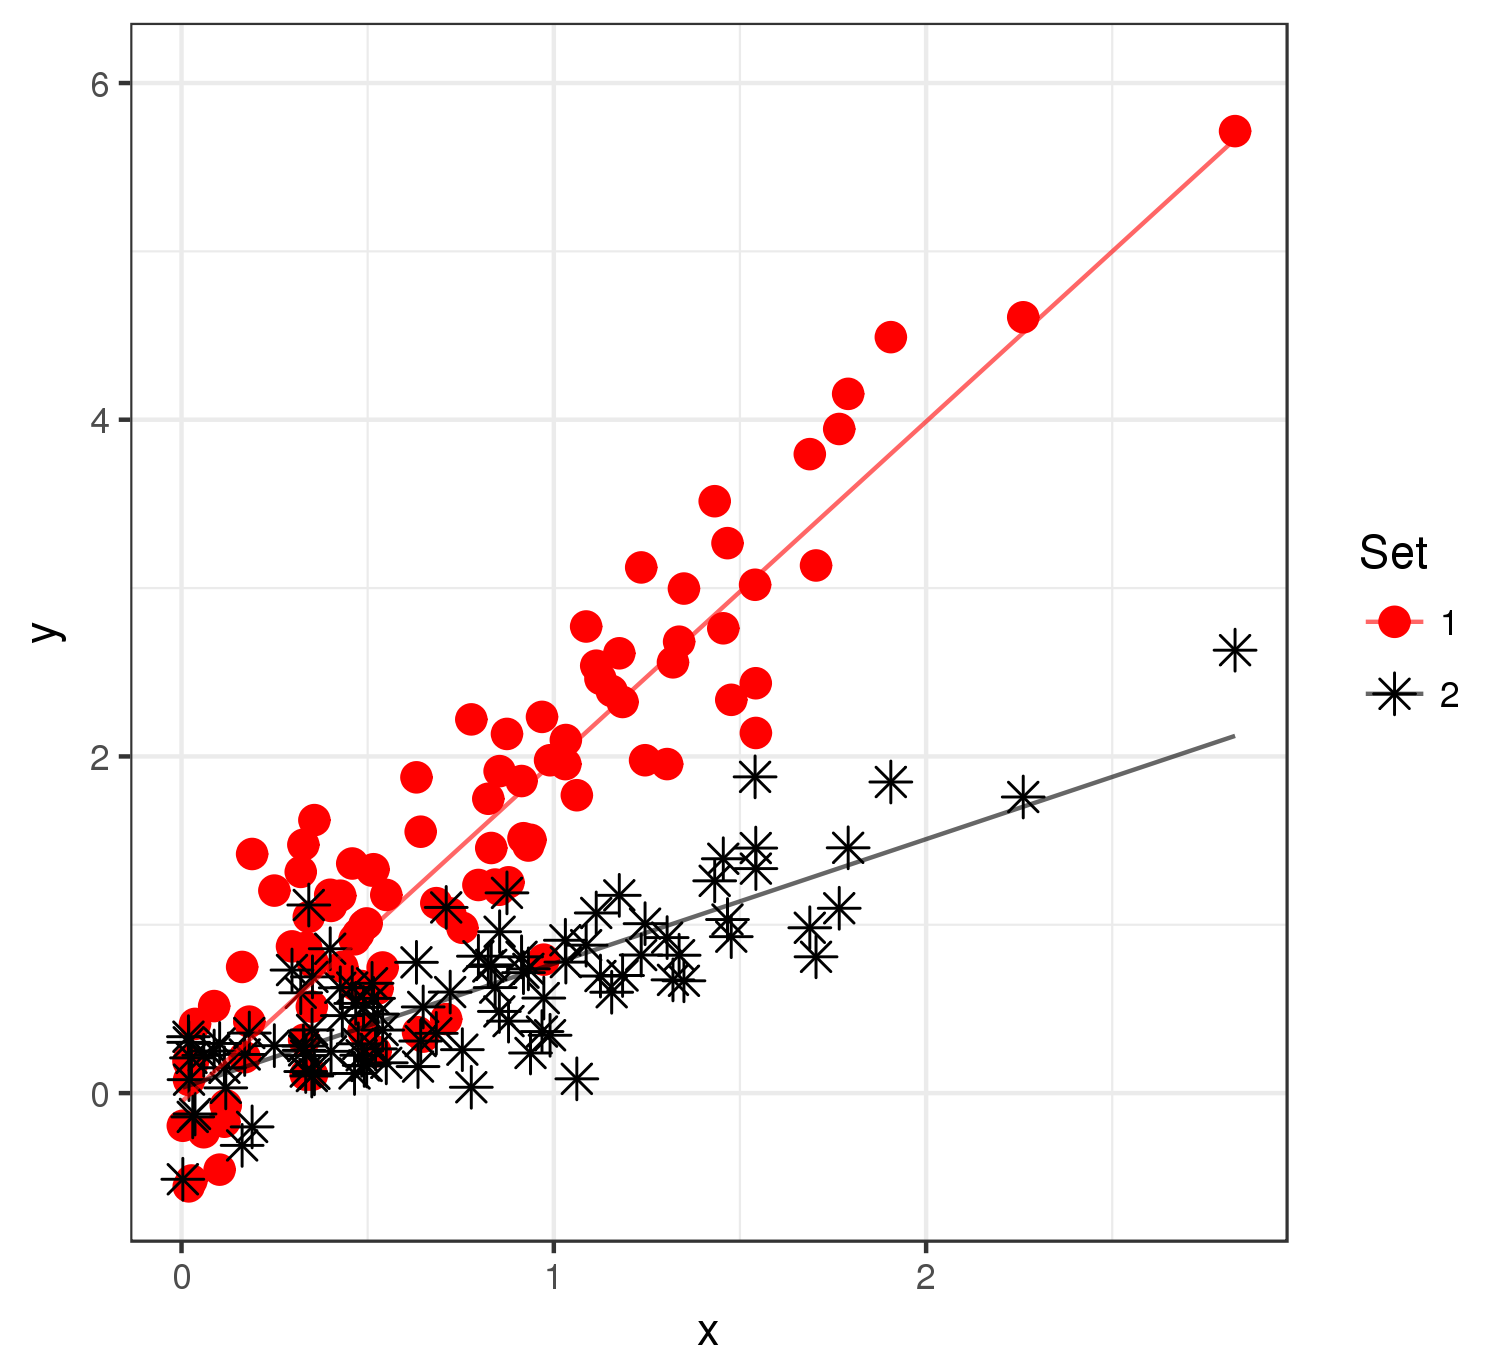
\includegraphics[width=1\linewidth]{fmr.png}
\caption{\footnotesize{}}\label{fig:sfig1}
\end{subfigure}
\begin{subfigure}{.5\textwidth}
\centering
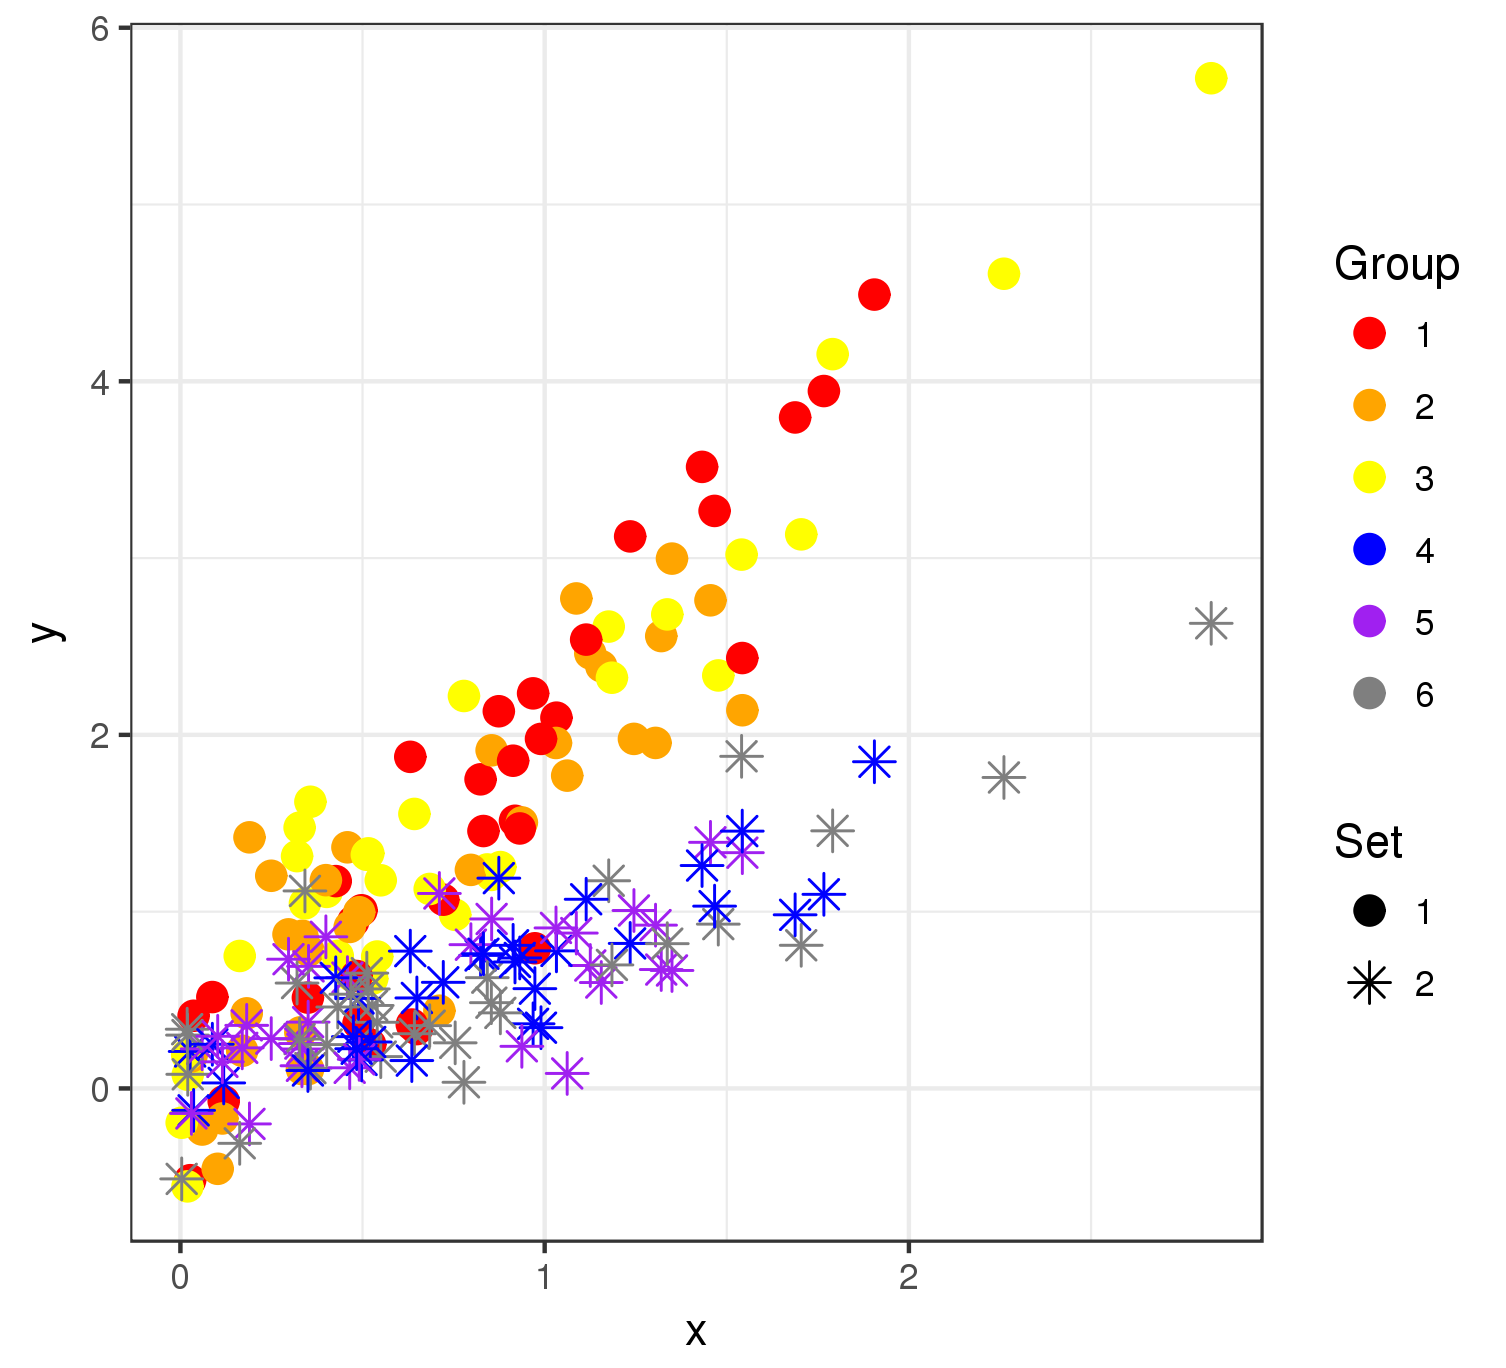
\includegraphics[width=1\linewidth, scale = 0.7]{fmr_const.png}

\caption{\footnotesize{}}\label{fig:sfig2}
\end{subfigure}
\caption{FMR with "must-link" constraint: (a) Synthetic, two component FMR without any constraint. (b) The same data points being divided into six groups where each group has to retain its data points.}\label{fig:fig1}
\end{figure}

To the best of our knowledge, all the existing algorithms have solved the problem of clustering with must-link constraint in unsupervised/semi-supervised settings, meaning that the observations lack (or partially lack) the dependent variable. In other words, we couldn't find any work that addresses the issue of model based clustering using FMMs \aaa{What is FMM?} with must-link constraint.

\subsection{Grouped mixture of regression}\label{sec:model}
\aaa{Major changes in this section...}
We assume that the observations belong to $R$ \emph{known groups}, denoted with labels $[R] := \{1,\dots,R\}$. In each group $r \in [R]$, we observe $n_r$ samples $(y_{ri},x_{ri}), i=1,\dots,n_r$ where $y_{ri} \in \reals$ is the response variable and $x_{ri} \in \reals^p$ is the vector of covariates or features.  We will write $x_{rij}$ to denote the $j^{th}$ feature in the feature vector $x_{ri}$. For the most part, we will treat $x_{ri}$ as deterministic observations, i.e., we have fixed design regression models.

We assume that there are $K$ latent (unobserved) clusters such that all the observations in group $r$ belong to that cluster. Thus, we can assign a cluster membership variable $z_{r} \in \{0,1\}^K$ to each group $r \in [R]$. We will have $z_{rk} = 1$ iff group $r$ belongs to cluster $k$.  With some abuse of notation, we also write $z_r = k$ in place of $z_{rk} = 1$.
%
%Let $D$ be the set of all data points, and $R$ be the total number of  distinct groups within $D$. Define $S$ as the set that holds all the group members and $X_r$ to represent a group: $S=\{X_r\}_{r=1}^{R}$. 
%Each group $X_r$, with $n_r$ observations, has to retain its members when assigned to a cluster. The goal is to assign each $X_r$ to one of $K$ clusters. Let's denote the whole data by $X$, $X = (X_1, \dots, X_R)^T$. We assume that the number of clusters ($K$) is known. 
%
%Let $x_{rij} \in {\rm I\!R}^p$ denote an observation  in $r^{th}$ group, $j^{th}$ column, and $i^{th}$ row in group $X_r$. Also, let $y_{ri} \in {\rm I\!R}$ denote the $i^{th}$ target variable in $r^{th}$ group, and $z_{rk}$ denote the latent (hidden) variable. $z_{rk}$ is an indicator for whether group $r$ belongs to component $k \in {\{1,\dots,K\}}$, and the vector $z_r := (z_{r1}, \dots z_{rk})^T$. Note that if we denote $Z$ as the collection of $z_{r}$'s: $Z := (z_{1}, \dots z_{R})^T$, then $Z$ will be a $R.K$ matrix with zeros and ones and contains the groups $r \in{\{1,\dots,R\}}$ in its rows, and the components $k\in{\{1, \dots,K\}}$ in its columns. In this case, there will be a single 1 in each row of $Z$, indicating the component that group $r$ belongs to. Finally, let $\theta = (\beta,\pi,\sigma^2)$ be the collection of all the parameters to be estimated.
%
%
%\section{EM for Mixture of Regression with Grouping Structure}
%\section{The model} 
Given the cluster membership variable $z_r$, we assume that the group $r$ observations are independent draws from a Gaussian linear regression model with parameters specified by $z_r$, that is,
\begin{align}\label{eq:gauss:mixreg:model}
	p(y_{ri} \cond z_{r} = k) \stackrel{\text{indept}}{\sim } N( \beta_k^T x_{ri}, \sigma_r^2), \; i =1,\dots,n_r,
\end{align}
where $\beta_k \in \reals^p$ is the coefficient vector the $k^{th}$ regression model and $\sigma_r^2$ is the noise variance for group $r$. Note that we are assuming that the noise level only depends on the group and not on the underlying cluster. \aaa{Might need some justification.} We write $\beta = (\beta_1 \mid \dots \mid \beta_K) \in \reals^{p \times K}$ and $\sigma^2 = (\sigma_1^2,\dots,\sigma_R^2) \in \reals^R$.

%Given the clusters that they belong to ($z_{rk}$),  the dependent variables ($y_{ri}$) in a particular group follow a Gaussian distribution with mean $ \beta_k^T x_{ri}$, which is the estimation of $y$ using the regression model for group $r$, and variance $\sigma_r^2$. That is: 

As is common in mixture modeling, we assume that $z_r$ follows a multinomial prior with parameter $\pi = (\pi_k)$, that is, $\pr(z_r = k) = \pi_k$ for $k \in [K]$, and $z_1,\dots,z_R$ are drawn independently.
%
%\noindent
%Here, we assume that the observations of dependent variable in a group $r$ are independent. Moreover, it is assumed that $z_r
%$ is a random variables that follows a Multinomial distribution with parameter $\pi_k$: 
%\begin{align}
%	z_r \sim \Mult(\pi_k), \quad \text{that is},\; \pr(z_r = k) = \pi_k
%	%z_{rk} = 1\{z_r = k\}\text{,} \; \text{and} \; \pi_k = P_\theta(z_r = k)
%\end{align}
The joint distribution of $y_r$ and $z_r$ is then given by:
%To apply EM to this setup, we first derive the joint distribution of $y_r$ and $z_r$:
\begin{align}
	p_{\theta}(y_r,z_r) = p_\theta(z_r) \prod_{i=1}^{n_r} p_\theta(y_{ri} \cond z_r) 
	= \prod_{k=1}^K \Big[\pi_k \prod_{i=1}^{n_r} p_\theta(y_{ri} \cond z_r = k)\Big]^{z_{rk}}
\end{align}
where we have let $\theta = (\beta,\pi,\sigma^2)$ collect all the parameters of the model.
%We also assume that $y_{ri}$ given $z_r$ are conditionally independent.
From~\eqref{eq:gauss:mixreg:model}, we have % We can write the conditional distributrion of $y_{ri}$ given $z_r$ as:
$p_\theta(y_{ri} \cond z_r = k) = \phi\big( (y_{ri} - \beta_k^T x_{ri})/\sigma_r \big)$, where $\phi(\cdot)$ is the density of the standard Gaussian distribution.
%\begin{align}
%	 p_\theta(y_{ri}|z_r = k) = \phi\Big( \frac{y_{ri} - \beta_k^T x_{ri}}{\sigma_r} \Big)
%\end{align}
Therefore, the so-called complete likelihood of $\theta$ given $(z,y)$ is:
\begin{align}\label{eq:likelihod}
	L(\theta \cond  y, z)= p_\theta(y,z) = \prod_{r=1}^R p_{\theta}(y_r,z_r) = \prod_{r=1}^R \prod_{k=1}^K \Big[\underbrace{\pi_k \prod_{i=1}^{n_r} \phi\Big( \frac{y_{ri} - \beta_k^T x_{ri}}{\sigma_r} \Big)}_{ =: \; \gamma_{rk}(\theta)} \Big]^{z_{rk}}
\end{align}
The parameter $\gamma_{rk}(\theta)$ in~\eqref{eq:likelihod} is proportional (in $k$) to the posterior probability of $z_r$ given the observation $y_r$, that is, $p_\theta(z_r = k \cond y_r) \propto_k p_\theta(y_r,z_r = k ) = \gamma_{rk}(\theta)$. By normalizing $\gamma_{rk}(\theta)$ over $k$, we obtain the \emph{posterior probability of cluster assignments}:
\begin{align}\label{eq:posterior:memebership}
	p_\theta(z_r = k \cond y_r) = \frac{\gamma_{rk}(\theta)}{\sum_{k'} \gamma_{rk'}(\theta)} =: \tau_{rk}(\theta), \quad 
\end{align}
for any $k \in [K]$ and $r \in [R]$. 
We note that the overall posterior factorizes over groups, i.e., $p_\theta(z \cond y) = \prod_{r} p_\theta(z_r \cond y_r)$, so it is enough to specify it for each pair $z_r$ and $y_r$. Thus, $\tau_{rk}(\theta)$ is the posterior probability that group $r$ belongs to cluster $k$, given all the observations $y$. These posterior probabilities are  key estimation objectives. 

 % , that is, $p_\theta(z_r = k|y_r) \propto_k \gamma_{rk}(\theta)$.
%
An estimate  $\thh = (\beh, \pih, \sigh^2)$ of $\theta$ can be obtained by maximizing~\eqref{eq:likelihod}. The classical approach to performing such optimization is by the Expectation Maximization (EM) algorithm, the details of which will be given in Section~?. Once we  have the estimate $\thh$ of the parameters, we can calculate an estimate of the posterior probabilities as $\tau_{rk}(\thh)$. 

\newcommand{\xnew}[1]{x_{#1,\text{new}}}
\newcommand{\ynew}[1]{y_{#1,\text{new}}}
\newcommand{\xtr}{x^{\text{train}}}
\newcommand{\ytr}{y^{\text{train}}}
\subsubsection{Prediction}
Now assume that we have new test data point $(\ynew{r},\xnew{r})$ in group $r$, for which we observe only the feature vector $\xnew{r}$ and would like to predict $\ynew{r}$. Let $(\ytr,\xtr)$ denote all the observations used in the training. The common link between the training and test data points are the latent variables $z_1,\dots,z_R$. In other words, since  we already have a good estimate of the membership of group $r$ based on the training data (via the posterior~\eqref{eq:posterior:memebership}), we can get a much better prediction of $\ynew{r}$ than what the prior model suggests. 
More precisely, we have the following \emph{predictive density} for $\ynew{r}$ based on $\ytr$,
%Let us compute the predictive density $p(\ynew{r}\cond \ytr)$. We have
\begin{align*}
	p_\theta(\ynew{r} \cond \ytr) &= \sum_{z_r} p_\theta(\ynew{r} \cond z_r) \;p_\theta(z_r \cond \ytr).
\end{align*}
Since, $p_\theta(z_r = k \cond \ytr) = p_\theta(z_r = k \cond \ytr_r) =\tau_{rk}(\theta)$, we obtain the following estimate of the predictive density
\begin{align}\label{eq:predict:post}
	p_{\thh}(\ynew{r} \cond \ytr)
	 = \sum_{k=1}^K p_\theta(\ynew{r}\cond z_r=k)\, \tau_{rk}(\thh) 
	=  \sum_{k=1}^K  \tau_{rk}(\thh) \,\phi\Big( \frac{\ynew{r} - \beh_k^T \xnew{r}}{\sigh_r} \Big).
\end{align}
Note that $\thh$ is our estimate of the parameters based on the training data  $(\ytr,\xtr)$.
In particular, the posterior mean based on~\eqref{eq:predict:post} is $\sum_{k=1}^K \tau_{rk}(\thh) \, \beh_k^T \xnew{r}$ which serves as the maximum a posterior (MAP) prediction for $\ynew{r}$.




\subsection{Estimation}

Let us now derive the EM updates for the model.
Recalling~\eqref{eq:likelihod}, the complete log-likelihood of the model is
\begin{align} \label{eq:loglik}
	\ell(\theta \cond  y, z) = \log  p_\theta(y,z) =  \sum_{r=1}^R \sum_{k=1}^K z_{rk} \Big[\log \pi_k + \sum_{i=1}^{n_r} \log \phi\Big( \frac{y_{ri} - \beta_k^T x_{ri}}{\sigma_r} \Big) \Big].
\end{align}



Treating the class latent memberships $\{z_r\}$ as missing data, we perform the EM updates to simultaneously estimate $\{z_r\}$ and $\theta$:
\begin{description}
\item[E-Step:] We replace~\eqref{eq:loglik} with its expectation under the approximate posterior of $\{z_r\}$:%, which we denote with $F(\theta;\thh)$. 
%We have   Since the log likelihood (equation ~\eqref{eq:loglik}) can't be maximized directly, it is replaced by its expectation ($F(\theta;\thh)$), given by ~\eqref{eq:exp_lik}:
\begin{align} 
\begin{split} \label{eq:exp_lik}
	F(\theta;\thh) := E_{z \sim \tau(\thh)} [\ell(\theta \cond y, z)] &=   \sum_{r=1}^R \sum_{k=1}^K \tau_{rk}(\thh) \Big[\log \pi_k + \sum_{i=1}^{n_r} \log \phi\Big( \frac{y_{ri} - \beta_k^T x_{ri}}{\sigma_r} \Big) \Big]\\
	&=\sum_{k=1}^K \tau_{+k}(\thh) \log \pi_k + 
	\sum_{r=1}^R \sum_{k=1}^K \sum_{i=1}^{n_r}  \tau_{rk}(\thh) \log \phi\Big( \frac{y_{ri} - \beta_k^T x_{ri}}{\sigma_r} \Big)
\end{split}
\end{align}
where $\tau_{rk}(\theta)$ is the posterior given in~\eqref{eq:posterior:memebership}, 
$ \tau_{+k}(\theta) = \sum_r \tau_{rk}(\theta)$. % and $\phi_\sigma(t) = \frac1{\sqrt{2\pi \sigma^2}} \exp(-t^2/2\sigma^2)$. 
%This is equivalent to computing the posterior probability of $z_r$ given $y_r$ ($\tau_{rk}(\theta)$), given the current estimate of the $\theta$.
\item[M-Step:] We then maximize $F(\theta;\thh)$ over $\theta$, giving the update rule for the parameters $\theta = (\beta,\pi,\sigma^2)$.%, and is achieved by setting the derivative of ~\eqref{eq:exp_lik2} to zero and solving for each of $\beta,\pi$, and $\sigma^2$. 
\end{description}

\begin{algorithm}[t!]
	\setstretch{1.2}
	\caption{Grouped mixture of regression (GMR)}\label{alg:gmr}
	\label{Palgorithm}
	\begin{algorithmic}[1]
		\State \makebox[3.25in][l]{Compute feature covariances for each group:  }
		$\Sigh_r \gets \frac1{n_r}\sum_{i=1}^{n_r} x_{ri} x_{ri}^T$
		
		\State \makebox[3.25in][l]{Compute feature-response  cross-covariances:  }
		$\rhoh_r \gets  \frac1{n_r}\sum_{i=1}^{n_r} y_{ri} x_{ri}$
		
		\State For any class posterior $\tau = (\tau_{rk})$ define the following weights:
		\begin{align*}
		\tau_{+k}(\tau) := \sum_r \tau_{rk}, 
		\quad w_{rk}(\tau) :=  n_r \tau_{rk},
		\quad  w_{+k}(\tau) := \sum_r  w_{rk},
		\quad \wc_{rk}(\tau) :=  \frac{w_{rk}}{w_{+k}}.
		\end{align*}
		and the weighted covariances: $\Sigt_k(\tau) := \sum_{r=1}^R \wc_{rk} \Sigh_r$ and 
		$\rhot_k(\tau) := \sum_{r=1}^R \wc_{rk}  \rhoh_r$.
		
		
		\State For any parameter $\theta = (\pi,\beta,\sigma^2)$ and class posterior $\tau = (\tau_{rk})$, define the errors:
		\begin{align*}
		E_{rk}(\beta) := \frac1{n_r}\sum_{i}^{n_r}   (y_{ri} - \beta_k^T x_{ri})^2, \quad 
		\Eb_k(\beta,\tau) := \sum_r \wc_{rk}(\tau) E_{rk}(\beta)
		\end{align*}
		
		\While{not converged}
		\State \makebox[2.25in][l]{Update class frequencies: }
		$\pi_k \gets \tau_{+k}(\tau)/R, \quad k \in [K] $
		
		\State \makebox[2.25in][l]{Update regression coefficients: }
		$\beta_k \gets \Sigt_k^{-1}(\tau) \,\rhot_k(\tau),\quad  k \in [K] $
		
		\State \makebox[2.25in][l]{Update noise variances: }
		$\sigma^2_k \gets \Eb_k(\beta, \tau), \quad k \in [K]$
		
		\EndWhile
	\end{algorithmic}
	
\end{algorithm}

To derive the update rules, we maximize $F(\theta;\thh)$ by a sequential block coordinate ascent, in each step maximizing  over one of the three sets of parameters $\pi, \beta$ and $\sigma^2$, while fixing the others. The updates are summarized in Algorithm~\ref{alg:gmr}. The details can be found in Appendix~\ref{sec:EM:details}.



\section{Empirical analysis}
\subsection{Synthetic data simulations}
To evaluate the effectiveness of the EM algorithm for FMR with group structure constraints, we employ Monte Carlo simulation experiments.
\subsection{Experiment Setup}
Table~\ref{tab:exp} summarizes the varying parameters that is used for the simulation.
Covariates ($X \in {\rm I\!R}^p$) for each component are generated by drawing samples from a multivariate Gaussian distribution:  $X \sim  \mathcal{N}(\boldsymbol{{\mu}} , \boldsymbol{{\Sigma}})$, with $\boldsymbol{\mu}=\overrightarrow{0}$.
\begin{table}[!htbp]
\centering
\caption{Monte Carlo Simulation Parameters}\label{tab:exp}
\begin{tabular}{|l|l|l|l|l|l|}
\hline
K & d      & S                   & N                                           & Noise Level                       & $\beta$ distance               \\ \hline
2 & 2      & \multirow{2}{*}{10} & \multirow{2}{*}{(100, 200, 400, 800, 1600)} & \multirow{2}{*}{(2, 4, 6, 8, 10)} & \multirow{2}{*}{(4, 7, 11)} \\ \cline{1-2}
4 & (2, 4) &                     &                                             &                                   &                             \\ \hline
\end{tabular}
\end{table}

Referring to table 1, $K$ is the number of components, $d$ is the dimension of independent variables ($p$), $S$ is the number of groups per component, and N is the total number of observations per component. As an example, there will be 10 observations per group for the case of N = 100, and 160 observations per group for when N = 1600. The response variable for each observation is generated by: $y_i= {X_i}^{'}\beta+Noise\; level$ . The "Noise level" is used as an indicator for the amount of noise (uncertainty) added to the response variable $y$.

To study the effect of the degree of similarity between $\beta$s, depending on the experiment (choise of $K$ and $d$), we generated $K$ number of $d$ dimensional equidistant points. The points are selected from (hyper)sphere in a way that they all have equal norm and equal pairwise distant, e.g. for the case of $K=42$, $\left| \left| \beta _{1}\right| \right|= \left| \left|\beta _{2}\right| \right|= \left| \left|\beta _{3}\right| \right| = \left| \left|\beta _{4}\right| \right|$, and $\left| \left| \beta _{1}-\beta _{2}\right| \right| ^{2}= \left| \left| \beta _{1}-\beta _{3}\right| \right| ^{2} = \left| \left| \beta _{1}-\beta _{4}\right| \right| ^{2} = \left| \left| \beta _{2}-\beta _{3}\right| \right| ^{2} = \left| \left| \beta _{2}-\beta _{4}\right| \right| ^{2} = \left| \left| \beta _{3}-\beta _{4}\right| \right| ^{2}= "\beta \text{ distance}"$. Generating $\beta$s this wa enables us to calculate and compare the estimation error among different runs in a single experiment setup. The comparison can be carried out across different experiment setups by normalizing the calculated error, e.g. by the "$\beta$ distance".
Three (3) "$\beta$ distance" values that are found to be sufficient for our purpose are selected (as shown in table~\ref{tab:exp}). Obviously, the smaller the distance, the closer the $\beta$s, and it is harder to separate the clusters.

\subsection{Evaluation Criterion}
The Monte Carlo simulations are repeated 1000 times for each pair of $\beta$ distance and Noise level as well as pairs of d and K. Four criterion are used to benchmark the performance of the algorithm.
\begin{itemize}
\item Normalized Mutual Information (NMI): NMI is used for assessing the clustering accuracy. NMI is a widely used technique in evaluating the clustering result when the true labels are available. The advantage of using NMI is that it is independent of permutation, meaning that the label switching does not affect the NMI score. It is bounded between zero and one. The closer the value to zero, the higher the indication that the cluster assignments are largely independent, while NMI close to one shows substantial agreement between the clusters. An NMI value of zero simply means that the label assignment is purely random.
\item $\beta$ estimation error: To calculate the error for estimating the coefficients of the components, we calculate the distance between the true and estimated $\beta$ by considering the miss-classification error as well. Let $C_k$ denote the (true) class $k$, and $\hat{C_r}$ denote the estimated class for group $r$. Equation \eqref{eq:bet_err} explains our approach:
\begin{align}\label{eq:bet_err}
\frac1n \sum_{i=1}^n \| \hat\beta^{(i)} - \beta^{(i)} \|^2 
		&=\frac1n \sum_{i=1}^n\Big[
		\sum_{r,k=1}^K  1\{ i \in C_k,  i \in \hat  C_r\}\Big] 
		\| \hat\beta^{(i)} - \beta^{(i)} \|^2\\
		&= \sum_{r,k=1}^K 	\frac1n \sum_{i=1}^n \Big[1\{ i \in C_k,  i \in \hat  C_r\}\Big]
	\| \hat\beta^{(i)} - \beta^{(i)} \|^2 \\
		&= \sum_{r,k=1}^K 	\frac1n \sum_{i=1}^n 1\{ i \in C_k,  i \in \hat  C_r\}\Big] 
		\| \hat\beta_r - \beta_k \|^2 \\
	   &=	 \sum_{r,k=1}^K 	\| \hat\beta_r - \beta_k \|^2	\frac1n \sum_{i=1}^n 1\{ i \in C_k,  i \in \hat  C_r\}\Big] 
	   \\ &= \sum_{r,k=1}^K 	\| \hat\beta_r - \beta_k \|^2 R_{kr} \\
	   &= \text{trace}(D^T R) = \sum_{k,r} D_{kr} R_{kr}	  
\end{align}
\noindent 
where $R$ is the confusion matrix divided by $n$ (number of observations), and $D$ is the matrix that holds pairwise distance between $\beta$s. 
\item Number of iterations: To study the rate of convergence and speed of the algorithm.
\item Root Mean Squared Error (RMSE): To evaluate the prediction power of the models, the models are used to predict a testing dataset. RMSE of the testing dataset is reported. 
\end{itemize}
 
 
\section{Result}
In this section a detailed discussion about the result of the simulation is presented. Each factor of the study is presented in a sub-section.


\begin{landscape}
% Please add the following required packages to your document preamble:
% \usepackage{booktabs}
% \usepackage{multirow}
\begin{table}[]
\centering
\caption{NMI}
\label{my-label}
\begin{tabular}{@{}cc|ccccc|ccccc|ccccc|@{}}
\cmidrule(l){3-17}
                                                     &                  & \multicolumn{5}{c|}{$\beta$ dist. = 4}                          & \multicolumn{5}{c|}{$\beta$ dist. = 7}                          & \multicolumn{5}{c|}{$\beta$ dist. = 11}                         \\ \cmidrule(l){2-17} 
\multicolumn{1}{c|}{}                                & {\textbf{%\backslashbox
                                                    {N} {Noise}}} & \textbf{2} & \textbf{4} & \textbf{6} & \textbf{8} & \textbf{10} & \textbf{2} & \textbf{4} & \textbf{6} & \textbf{8} & \textbf{10} & \textbf{2} & \textbf{4} & \textbf{6} & \textbf{8} & \textbf{10} \\ \midrule
\multicolumn{1}{|c|}{\multirow{4}{*}{\rotatebox{90}{K = 2; d = 2}}} & \textbf{100}     & 0.88       & 0.43       & 0.22       & 0.13       & 0.09        & 0.99       & 0.87       & 0.62       & 0.43       & 0.27        & 0.99       & 0.98       & 0.88       & 0.71       & 0.54        \\
\multicolumn{1}{|c|}{}                               & \textbf{200}     & 0.98       & 0.71       & 0.40       & 0.25       & 0.15        & 0.99       & 0.98       & 0.88       & 0.68       & 0.54        & 1          & 0.99       & 0.97       & 0.92       & 0.82        \\
\multicolumn{1}{|c|}{}                               & \textbf{400}     & 0.99       & 0.91       & 0.68       & 0.46       & 0.32        & 1          & 0.99       & 0.98       & 0.90       & 0.81        & 1          & 1          & 0.99       & 0.98       & 0.96        \\
\multicolumn{1}{|c|}{}                               & \textbf{800}     & 1          & 0.99       & 0.98       & 0.90       & 0.75        & 1          & 1          & 1          & 0.99       & 0.99        & 1          & 1          & 1          & 1          & 1           \\ \midrule
\multicolumn{1}{|c|}{\multirow{4}{*}{\rotatebox{90}{K = 2; d = 4}}} & \textbf{100}     & 0.93       & 0.49       & 0.21       & 0.13       & 0.09        & 0.99       & 0.93       & 0.73       & 0.48       & 0.32        & 0.99       & 0.99       & 0.93       & 0.8        & 0.64        \\
\multicolumn{1}{|c|}{}                               & \textbf{200}     & 0.99       & 0.82       & 0.45       & 0.26       & 0.16        & 1          & 0.99       & 0.94       & 0.80       & 0.62        & 1          & 0.99       & 0.99       & 0.97       & 0.91        \\
\multicolumn{1}{|c|}{}                               & \textbf{400}     & 1          & 0.97       & 0.79       & 0.54       & 0.35        & 1          & 1          & 0.99       & 0.97       & 0.89        & 1          & 1          & 1          & 0.99       & 0.99        \\
\multicolumn{1}{|c|}{}                               & \textbf{800}     & 1          & 0.99       & 0.96       & 0.84       & 0.64        & 1          & 1          & 1          & 0.99       & 0.98        & 1          & 1          & 1          & 1          & 0.99        \\ \midrule
\multicolumn{1}{|c|}{\multirow{4}{*}{\rotatebox{90}{K = 4; d = 4}}} & \textbf{100}     & 0.80       & 0.34       & 0.20       & 0.15       & 0.12        & 0.97       & 0.80       & 0.52       & 0.34       & 0.25        & 0.98       & 0.94       & 0.81       & 0.62       & 0.45        \\
\multicolumn{1}{|c|}{}                               & \textbf{200}     & 0.95       & 0.61       & 0.33       & 0.21       & 0.17        & 0.97       & 0.95       & 0.81       & 0.61       & 0.44        & 0.97       & 0.97       & 0.95       & 0.86       & 0.75        \\
\multicolumn{1}{|c|}{}                               & \textbf{400}     & 0.96       & 0.86       & 0.58       & 0.38       & 0.27        & 0.96       & 0.96       & 0.94       & 0.86       & 0.72        & 0.96       & 0.96       & 0.96       & 0.95       & 0.92        \\
\multicolumn{1}{|c|}{}                               & \textbf{800}     & 0.95       & 0.95       & 0.84       & 0.64       & 0.47        & 0.95       & 0.95       & 0.96       & 0.95       & 0.92        & 0.96       & 0.95       & 0.96       & 0.96       & 0.96        \\ \bottomrule
\end{tabular}
\end{table}
\end{landscape}

\begin{landscape}
% Please add the following required packages to your document preamble:
% \usepackage{booktabs}
% \usepackage{multirow}
\begin{table}[]
\centering
\caption{$\beta$ error}
\label{my-label}
\begin{tabular}{@{}ll|lllll|lllll|lllll|@{}}
\cmidrule(l){3-17}
                                                     &                                       & \multicolumn{5}{l|}{$\beta$ dist. = 4}                          & \multicolumn{5}{l|}{$\beta$ dist. = 7}                          & \multicolumn{5}{l|}{$\beta$ dist. = 11}                         \\ \cmidrule(l){2-17} 
\multicolumn{1}{l|}{}                                & {\textbf{%\backslashbox
                                                    {N} {Noise}}} & \textbf{2} & \textbf{4} & \textbf{6} & \textbf{8} & \textbf{10} & \textbf{2} & \textbf{4} & \textbf{6} & \textbf{8} & \textbf{10} & \textbf{2} & \textbf{4} & \textbf{6} & \textbf{8} & \textbf{10} \\ \midrule
\multicolumn{1}{|l|}{\multirow{4}{*}{\rotatebox{90}{K = 2; d = 2}}} & \textbf{100}                          & 0.79       & 0.96       & 1.07       & 1.19       & 1.42        & 0.77       & 0.81       & 0.85       & 0.90       & 1.03        & 0.8        & 0.78       & 0.79       & 0.85       & 0.93        \\
\multicolumn{1}{|l|}{}                               & \textbf{200}                          & 0.76       & 0.81       & 0.97       & 1.06       & 1.15        & 0.78       & 0.81       & 0.79       & 0.87       & 0.90        & 0.79       & 0.76       & 0.78       & 0.81       & 0.81        \\
\multicolumn{1}{|l|}{}                               & \textbf{400}                          & 0.79       & 0.76       & 0.85       & 0.96       & 1.02        & 0.79       & 0.79       & 0.8        & 0.82       & 0.85        & 0.78       & 0.79       & 0.76       & 0.81       & 0.79        \\
\multicolumn{1}{|l|}{}                               & \textbf{800}                          & 0.07       & 0.1        & 0.14       & 0.21       & 0.31        & 0.06       & 0.07       & 0.08       & 0.1        & 0.12        & 0.06       & 0.06       & 0.07       & 0.08       & 0.09        \\ \midrule
\multicolumn{1}{|l|}{\multirow{4}{*}{\rotatebox{90}{K = 2; d = 4}}} & \textbf{100}                          & 0.21       & 0.59       & 0.95       & 1.19       & 1.41        & 0.11       & 0.59       & 0.38       & 0.59       & 0.78        & 0.09       & 0.14       & 0.21       & 0.32       & 0.45        \\
\multicolumn{1}{|l|}{}                               & \textbf{200}                          & 0.14       & 0.32       & 0.63       & 0.88       & 1.06        & 0.09       & 1.43       & 0.21       & 0.32       & 0.47        & 0.08       & 0.11       & 0.14       & 0.18       & 0.25        \\
\multicolumn{1}{|l|}{}                               & \textbf{400}                          & 0.11       & 0.19       & 0.35       & 0.55       & 0.76        & 0.08       & 0.10       & 0.14       & 0.19       & 0.26        & 0.07       & 0.09       & 0.11       & 0.13       & 0.16        \\
\multicolumn{1}{|l|}{}                               & \textbf{800}                          & 0.09       & 1.40       & 0.20       & 0.31       & 0.46        & 0.07       & 0.09       & 0.11       & 0.13       & 0.17        & 0.06       & 0.07       & 0.09       & 0.10       & 0.12        \\ \midrule
\multicolumn{1}{|l|}{\multirow{4}{*}{\rotatebox{90}{K = 4; d = 4}}} & \textbf{100}                          & 1.17       & 1.3        & 1.44       & 1.60       & 1.76        & 1.12       & 1.17       & 1.23       & 1.3        & 1.38        & 1.13       & 1.14       & 1.41       & 1.62       & 1.83        \\
\multicolumn{1}{|l|}{}                               & \textbf{200}                          & 1.14       & 1.23       & 1.31       & 1.40       & 1.51        & 1.14       & 1.15       & 1.17       & 1.20       & 1.26        & 1.13       & 1.12       & 1.15       & 1.16       & 1.19        \\
\multicolumn{1}{|l|}{}                               & \textbf{400}                          & 1.14       & 1.13       & 1.21       & 1.29       & 1.36        & 1.13       & 1.13       & 1.16       & 1.16       & 1.19        & 1.13       & 1.14       & 1.13       & 1.14       & 1.15        \\
\multicolumn{1}{|l|}{}                               & \textbf{800}                          & 1313       & 1.14       & 1.16       & 1.21       & 1.25        & 1.13       & 1.13       & 1.14       & 1.14       & 1.14        & 1.14       & 1.13       & 1.13       & 1.14       & 1.14        \\ \bottomrule
\end{tabular}
\end{table}
\end{landscape}

\begin{landscape}
% Please add the following required packages to your document preamble:
% \usepackage{booktabs}
% \usepackage{multirow}
\begin{table}[]
\centering
\caption{RMSE}
\label{my-label}
\begin{tabular}{@{}ll|lllll|lllll|lllll|@{}}
\cmidrule(l){3-17}
                                                     &                                       & \multicolumn{5}{l|}{$\beta$ distance = 4}                       & \multicolumn{5}{l|}{$\beta$ distance = 7}                       & \multicolumn{5}{l|}{$\beta$ distance = 11}                      \\ \cmidrule(l){2-17} 
\multicolumn{1}{l|}{}                                & {\textbf{%\backslashbox
                                                    {N} {Noise}}} & \textbf{2} & \textbf{4} & \textbf{6} & \textbf{8} & \textbf{10} & \textbf{2} & \textbf{4} & \textbf{6} & \textbf{8} & \textbf{10} & \textbf{2} & \textbf{4} & \textbf{6} & \textbf{8} & \textbf{10} \\ \midrule
\multicolumn{1}{|l|}{\multirow{4}{*}{\rotatebox{90}{K = 2; d = 2}}} & \textbf{100}                          & 1.49       & 2.12       & 2.87       & 3.71       & 4.54        & 1.23       & 1.48       & 1.77       & 2.10       & 2.49        & 1.2        & 1.30       & 1.47       & 1.67       & 1.88        \\
\multicolumn{1}{|l|}{}                               & \textbf{200}                          & 1.23       & 2.11       & 2.87       & 3.69       & 4.51        & 1.23       & 1.47       & 1.76       & 2.10       & 2.49        & 2.11       & 1.32       & 1.46       & 1.66       & 1.88        \\
\multicolumn{1}{|l|}{}                               & \textbf{400}                          & 1.46       & 2.11       & 2.88       & 3.68       & 4.52        & 1.25       & 1.48       & 1.78       & 2.13       & 2.48        & 2.98       & 1.32       & 1.46       & 1.66       & 1.89        \\
\multicolumn{1}{|l|}{}                               & \textbf{800}                          & 1.39       & 2.06       & 2.83       & 3.6        & 4.49        & 1.18       & 1.4        & 1.7        & 2.06       & 2.44        & 1.13       & 1.26       & 1.4        & 1.6        & 1.833       \\ \midrule
\multicolumn{1}{|l|}{\multirow{4}{*}{\rotatebox{90}{K = 2; d = 4}}} & \textbf{100}                          & 1.45       & 2.10       & 2.86       & 3.69       & 4.53        & 1.23       & 1.45       & 1.75       & 2.11       & 2.50        & 1.18       & 1.30       & 1.44       & 1.65       & 1.86        \\
\multicolumn{1}{|l|}{}                               & \textbf{200}                          & 1.45       & 2.10       & 2.87       & 3.68       & 4.51        & 1.23       & 1.45       & 1.75       & 2.10       & 2.48        & 1.19       & 1.30       & 1.45       & 1.64       & 1.86        \\
\multicolumn{1}{|l|}{}                               & \textbf{400}                          & 0.14       & 2.10       & 2.86       & 3.67       & 4.51        & 1.24       & 1.45       & 1.75       & 2.10       & 2.47        & 1.19       & 1.30       & 1.45       & 1.64       & 1.86        \\
\multicolumn{1}{|l|}{}                               & \textbf{800}                          & 1.44       & 2.09       & 2.86       & 3.67       & 4.50        & 1.23       & 1.45       & 1.74       & 2.09       & 2.46        & 1.19       & 1.29       & 1.45       & 1.65       & 1.86        \\ \midrule
\multicolumn{1}{|l|}{\multirow{4}{*}{\rotatebox{90}{K = 4; d = 4}}} & \textbf{100}                          & 1.41       & 2.07       & 2.85       & 3.67       & 4.50        & 1.18       & 1.41       & 1.72       & 2.07       & 2.45        & 1.14       & 1.25       & 1.41       & 1.62       & 1.83        \\
\multicolumn{1}{|l|}{}                               & \textbf{200}                          & 1.41       & 2.06       & 2.84       & 3.66       & 4.49        & 1.19       & 1.40       & 1.72       & 2.06       & 2.45        & 1.15       & 1.26       & 1.41       & 1.61       & 1.82        \\
\multicolumn{1}{|l|}{}                               & \textbf{400}                          & 1.41       & 2.07       & 2.84       & 3.66       & 4.50        & 1.19       & 1.41       & 1.72       & 2.06       & 2.44        & 1.14       & 1.25       & 1.41       & 1.60       & 1.83        \\
\multicolumn{1}{|l|}{}                               & \textbf{800}                          & 1.41       & 2.06       & 2.84       & 3.65       & 4.49        & 1.19       & 1.41       & 1.72       & 2.07       & 2.44        & 1.14       & 1.25       & 1.41       & 1.60       & 1.82        \\ \bottomrule
\end{tabular}
\end{table}
\end{landscape}

\begin{landscape}
% Please add the following required packages to your document preamble:
% \usepackage{booktabs}
% \usepackage{multirow}
\begin{table}[]
\centering
\caption{Number of iterations}
\label{my-label}
\begin{tabular}{@{}ll|lllll|llllllllll|@{}}
\cmidrule(l){3-17}
                                                     &                                       & \multicolumn{5}{l|}{$\beta$ distance = 4}                       & \multicolumn{5}{l}{$\beta$ distance = 7}                                             & \multicolumn{5}{l|}{$\beta$ distance = 11}                      \\ \cmidrule(l){2-17} 
\multicolumn{1}{l|}{}                                & {\textbf{%\backslashbox
                                                    {N} {Noise}}} & \textbf{2} & \textbf{4} & \textbf{6} & \textbf{8} & \textbf{10} & \textbf{2} & \textbf{4} & \textbf{6} & \textbf{8} & \multicolumn{1}{l|}{\textbf{10}} & \textbf{2} & \textbf{4} & \textbf{6} & \textbf{8} & \textbf{10} \\ \midrule
\multicolumn{1}{|l|}{\multirow{4}{*}{\rotatebox{90}{K = 2; d = 2}}} & \textbf{100}                          & 14.1       & 53.7       & 84.2       & 100.2      & 109.0       & 4.9        & 14.3       & 32.9       & 53.7       & \multicolumn{1}{l|}{71.3}        & 3.8        & 7.5        & 13.6       & 27.2       & 40.1        \\
\multicolumn{1}{|l|}{}                               & \textbf{200}                          & 6.3        & 27.6       & 60.6       & 82.4       & 101.3       & 3.3        & 6.4        & 14.4       & 29.3       & \multicolumn{1}{l|}{44.7}        & 3.1        & 3.8        & 6.6        & 11.5       & 19.6        \\
\multicolumn{1}{|l|}{}                               & \textbf{400}                          & 3.6        & 12.3       & 33.2       & 55.4       & 74.1        & 2.9        & 3.6        & 6.4        & 12.9       & \multicolumn{1}{l|}{20.4}        & 2.8        & 3.0        & 3.5        & 5.6        & 8.3         \\
\multicolumn{1}{|l|}{}                               & \textbf{800}                          & 2.7        & 3.4        & 6.8        & 13.9       & 24.7        & 2.5        & 2.8        & 3          & 3.4        & \multicolumn{1}{l|}{4.7}         & 2.4        & 2.6        & 2.8        & 2.9        & 3.1         \\ \midrule
\multicolumn{1}{|l|}{\multirow{4}{*}{\rotatebox{90}{K = 2; d = 4}}} & \textbf{100}                          & 11.4       & 42.8       & 65.1       & 72.4       & 73.6        & 4.2        & 12.1       & 25.2       & 43.2       & \multicolumn{1}{l|}{55.2}        & 3.6        & 5.8        & 12.0       & 19.6       & 30.8        \\
\multicolumn{1}{|l|}{}                               & \textbf{200}                          & 4.8        & 20.6       & 45.8       & 65.4       & 73.4        & 3.2        & 4.8        & 11.2       & 20.5       & \multicolumn{1}{l|}{32.8}        & 3.1        & 3.4        & 4.7        & 8.2        & 13.7        \\
\multicolumn{1}{|l|}{}                               & \textbf{400}                          & 3.2        & 8.8        & 23.3       & 42.5       & 57.5        & 2.9        & 3.2        & 4.7        & 8.6        & \multicolumn{1}{l|}{15.7}        & 2.8        & 3.0        & 3.2        & 3.8        & 5.7         \\
\multicolumn{1}{|l|}{}                               & \textbf{800}                          & 2.8        & 4.0        & 9.5        & 19.7       & 34.2        & 2.5        & 2.8        & 3.1        & 3.8        & \multicolumn{1}{l|}{6.1}         & 2.4        & 2.6        & 2.8        & 3.1        & 3.3         \\ \midrule
\multicolumn{1}{|l|}{\multirow{4}{*}{\rotatebox{90}{K = 4; d = 4}}} & \textbf{100}                          & 41.1       & 114.0      & 149.7      & 163.2      & 171.1       & 13.0       & 40.5       & 81.1       & 113.4      & \multicolumn{1}{l|}{134.1}       & 8.5        & 20.1       & 39.3       & 67.9       & 94.1        \\
\multicolumn{1}{|l|}{}                               & \textbf{200}                          & 18.6       & 74.7       & 121.8      & 149.1      & 162.5       & 7.7        & 18.3       & 42.7       & 72.8       & \multicolumn{1}{l|}{103.0}       & 9.15       & 10.7       & 18.5       & 33.2       & 52.3        \\
\multicolumn{1}{|l|}{}                               & \textbf{400}                          & 11.6       & 36.5       & 81.5       & 117.1      & 142.7       & 11.3       & 12.3       & 20.2       & 36.2       & \multicolumn{1}{l|}{59.8}        & 11.0       & 11.8       & 12.8       & 17.1       & 25.4        \\
\multicolumn{1}{|l|}{}                               & \textbf{800}                          & 12.7       & 18.1       & 40.5       & 72.8       & 104.6       & 13.0       & 13.2       & 12.0       & 17.8       & \multicolumn{1}{l|}{27.7}        & 10.1       & 12.6       & 12.7       & 12.5       & 14.0        \\ \bottomrule
\end{tabular}
\end{table}
\end{landscape}



%%%%%%%%%%%%%%%%%%%%%%%%%%%%%%%%%%%%%%%%%%%%%%%%%%%%%%%%%%%%%%%%%%%%%%%%%%%
\subsection{Dimension (d)}

\section{Case Study: Deriving Recommendations for Automotive Dealerships}

\subsection{Applying the Algorithm to the Dealership Performance Problem}


\subsubsection{Results}

\section{Conclusion}
\label{sec:conc}
\cleardoublepage
\begin{appendices}
\section{The EM updates}\label{sec:EM:details}
We have to calculate expectation under $p_\theta(z_r = k|y_r)$ to obtain:
\begin{align*}
	F(\theta;\thh) = E_{z \sim \tau(\thh)} [\ell(\theta;z)] &=   \sum_{r=1}^R \sum_{k=1}^K \tau_{rk}(\thh) \Big[\log \pi_k + \sum_{i=1}^{n_r} \log \phi\Big( \frac{y_{ri} - \beta_k^T x_{ri}}{\sigma_r} \Big) \Big]\\
	&=\sum_{k=1}^K \tau_{+k}(\thh) \log \pi_k + 
	\sum_{r=1}^R \sum_{k=1}^K \sum_{i=1}^{n_r}  \tau_{rk}(\thh) \log \phi\Big( \frac{y_{ri} - \beta_k^T x_{ri}}{\sigma_r} \Big)
\end{align*}


We would like to maximize (7) over $\theta$. Note that $\beta_k,x_{rk} \in \reals^p$ ($p$ is the number of covariates).
We will use $\doteq_\pi$ for example, when the two sides are equal upto additive constants, as functions of $\pi$. Fixing everything and maximizing over $\pi = (\pi_1,\dots,\pi_k)$, we are maximizing $\pi \mapsto \sum_k \tau_{+k}(\thh) \log \pi_k$ over probability vector $\pi$. This is the MLE in multinomial family and the solution is $\pi_k \propto_k \tau_{+k}$, that is
	\begin{align}\label{eq:pi:update:1}
	    \pi_k = \frac{\tau_{+k}}{\sum_{k'} \tau_{+k'}}  = \frac{\tau_{+k}}{R}
	\end{align}
	where we used $\sum_{k'} \tau_{+k'} = \sum_{k'} \sum_r \tau_{rk'} = \sum_r \sum_{k'} \tau_{rk'} = \sum_r 1 = R$, since for fixed $r$, $\tau_{rk}$ sums to 1 over $k$.
	
	To maximize over $\beta$, we again fix everything else. Since $\log \phi_\sigma(t) \doteq_t -\frac12 (\log \sigma^2 + t^2/\sigma^2) $, we are maximizing
	\begin{align}
	    F(\theta;\thh)\; &\doteq_\beta\; -\sum_r \sum_k \sum_i^{n_r} 
	    \tau_{rk}(\thh) \frac1{2\sigma_k^2} (y_{ri} - \beta_k^T x_{ri})^2 \\
	    &\doteq_\beta\; -\sum_r \sum_k \sum_i^{n_r} 
	    \tau_{rk}(\thh) \frac1{2\sigma_k^2} [(\beta_k^T x_{ri})^2 - 2y_{ri}\beta_k^T x_{ri}] \label{eq:temp:1}
	\end{align}
	ignoring constant terms generated by $y_{ri}^2$. Note that $(\beta_k^T x_{ri})^2 = (\beta_k^T x_{ri})(x_{ri}^T \beta_k) = \beta_k^T (x_{ri}x_{ri}^T) \beta_k$. Similarly, $y_{ri}\beta_k^T x_{ri} = \beta_k^T(y_{ri} x_{ri})$. Let us define
	\begin{align}\label{eq:hat:def}
	    \Sigh_r := \frac1{n_r}\sum_{i=1}^{n_r} x_{ri} x_{ri}^T, \quad 
	    \rhoh_r :=  \frac1{n_r}\sum_{i=1}^{n_r} y_{ri} x_{ri}
	\end{align}
	Summing over $i$ first in~\eqref{eq:temp:1}, we get
	\begin{align}
	     F(\theta;\thh)\; 
	    &\doteq_\beta\; -\sum_r \sum_k
	     \frac{\tau_{rk}}{2\sigma_k^2} n_r[ \beta_k^T \Sigh_r \beta_k - 2 \beta_k^T \rhoh_r] \notag \\
	    &=  - \sum_k \frac1{2\sigma_k^2}
	     \sum_r\tau_{rk} n_r[ \beta_k^T \Sigh_r \beta_k - 2 \beta_k^T \rhoh_r]
	     \label{eq:temp:2}
	\end{align}

	
	Let us define 
	\begin{align}\label{eq:w:def}
	    w_{rk} :=  n_r \tau_{rk}, \quad \wc_{rk} := \frac{w_{rk}}{w_{+k}}
	\end{align}
	 where $w_{+k} = \sum_r n_r\tau_{rk}$. Let
	\begin{align}\label{eq:tilde:def}
	    \Sigt_k := \sum_{r=1}^R \wc_{rk} \Sigh_r, \quad 
	    \rhot_k := \sum_{r=1}^R \wc_{rk}  \rhoh_r.
	\end{align}
	Dividing and multiplying by $w_{+k}$ and summing over $r$ in~\eqref{eq:temp:2}, we get
	\begin{align}
	    F(\theta;\thh)\; 
	    &\doteq_\beta\; -\sum_k \frac{w_{+k}}{2\sigma_k^2} [\beta_k^T \Sigt_k \beta_k - 2 \beta_k^T \rhot_k]
	\end{align}
	The problem is separable in $k$, and the minimizer over $\beta_k$ is
	\begin{align}
	    \beta_k = \Sigt_k^{-1} \rhot_k
	\end{align}

	\bigskip
	To optimize over $\alpha_k:=\sigma_k^2$, let us fix everything else. We have
	\begin{align}\label{eq:temp:495}
	    F(\theta;\thh) \doteq_{\alpha} -\frac12 \sum_k \Big[ \sum_r \sum_i^{n_r} \tau_{rk} \log \alpha_k + \sum_r \sum_i^{n_r} 
	    \tau_{rk}\frac{(y_{ri} - \beta_k^T x_{ri})^2}{\alpha_k}\Big]
	\end{align}
	The first term in brackets is
	 $(\sum_r n_r \tau_{rk}) \log \alpha_k = w_{+k} \log \alpha_k$. See~\eqref{eq:w:def}.
	%
	
	Defining
	\begin{align}
	    E_{rk} := E_{rk}(\beta) := \frac1{n_r}\sum_{i}^{n_r}   (y_{ri} - \beta_k^T x_{ri})^2, \qquad 
	    \Eb_k := \Eb_k(\beta) := \sum_r \wc_{rk} E_{rk}.
	\end{align}
	we see that the second term in brackets in~\eqref{eq:temp:495} is just $w_{+k}\Eb_k$. We have
	\begin{align}
	     F(\theta;\thh)   \doteq_{\alpha}
	     -\frac12 \sum_k w_{+k} \Big[  \log \alpha_k + \frac{\Eb_k}{\alpha_k}\Big]
	\end{align}
	This problem is separable in $\alpha_k$ and the solution is $\alpha_k = \Eb_k$.

	\medskip
	To summarize, we sequentially update the parameters ($\theta$) as follows ($[K] := \{1,\dots,K\}$)
	\begin{align}
	    \pi_k &= \tau_{+k}/R, \quad k \in [K] \\
	    \beta_k &= \Sigt_k^{-1} \rhot_k,\quad  k \in [K] \\
	    \sigma^2_k &= \Eb_k(\beta), \quad k \in [K]
	\end{align}
\end{appendices}

\begin{align}
	\frac1n \sum_{i=1}^n \| \hat\beta^{(i)} - \beta^{(i)} \|^2 
		&=\frac1n \sum_{i=1}^n\Big[
		\sum_{r,k=1}^K  1\{ i \in C_k,  i \in \hat  C_r\}\Big] 
		\| \hat\beta^{(i)} - \beta^{(i)} \|^2\\
		&= \sum_{r,k=1}^K 	\frac1n \sum_{i=1}^n \Big[1\{ i \in C_k,  i \in \hat  C_r\}\Big]
	\| \hat\beta^{(i)} - \beta^{(i)} \|^2 \\
		&= \sum_{r,k=1}^K 	\frac1n \sum_{i=1}^n 1\{ i \in C_k,  i \in \hat  C_r\}\Big] 
		\| \hat\beta_r - \beta_k \|^2 \\
	   &=	 \sum_{r,k=1}^K 	\| \hat\beta_r - \beta_k \|^2	\frac1n \sum_{i=1}^n 1\{ i \in C_k,  i \in \hat  C_r\}\Big] 
	   \\ &= \sum_{r,k=1}^K 	\| \hat\beta_r - \beta_k \|^2 R_{kr} \\
	   &= \text{trace}(D^T R) = \sum_{k,r} D_{kr} R_{kr}
\end{align}

\begin{align*}
	\frac1n \sum_{i=1}^n \| \hat\beta^{(i)} - \beta^{(i)} \|^2 
		&=\frac1n \sum_{i=1}^n\Big[
		\sum_{r,k=1}^K  1\{ i \in C_k,  i \in \hat  C_r\}\Big] 
		\| \hat\beta^{(i)} - \beta^{(i)} \|^2\\
	   &=	 \sum_{r,k=1}^K 	\| \hat\beta_r - \beta_k \|^2	\frac1n \sum_{i=1}^n 1\{ i \in C_k,  i \in \hat  C_r\}\Big] 
\end{align*}

\cleardoublepage

\small
\bibliographystyle{Chicago}

\bibliography{bibfile}
\end{document}



